\documentclass{templateReport}
\usepackage{tocloft} % Para personalizar el índice de contenidos

% Algunos colores personalizados
\definecolor{Violeta}{RGB}{124,0,254}
\definecolor{Verde2}{RGB}{130,254,0} % Complementario
\definecolor{Naranja2}{RGB}{254,124,0} % Triadico
\definecolor{Verde3}{RGB}{0,254,124} % Triadico

\definecolor{Amarillo}{RGB}{249,228,0}
\definecolor{Azul2}{RGB}{0,21,249} % Complementario
\definecolor{Celeste2}{RGB}{0,249,228} % Triadico
\definecolor{Rosa}{RGB}{228,0,249} % Triadico

\definecolor{Naranja}{RGB}{255,175,0}
\definecolor{Azul3}{RGB}{0,80,255} % Complementario
\definecolor{Cian}{RGB}{0,255,175} % Triadico
\definecolor{Violeta2}{RGB}{175,0,255} % Triadico

\definecolor{Rojo}{RGB}{245,0,79}
\definecolor{Verde4}{RGB}{0,245,166} % Complementario
\definecolor{Verde}{RGB}{79,245,0} % Triadico
\definecolor{Azul}{RGB}{0,79,245} % Triadico

\definecolor{Celeste}{RGB}{0,191,255}
\definecolor{Salmon}{RGB}{255,0,157}

\newcommand{\newparagraph}{\par\vspace{\baselineskip}\noindent}
\newcommand{\hlcolor}[2]{{\sethlcolor{#1}\hl{#2}}}

% Personalizar el formato del índice de contenidos
\addto\captionsspanish{\renewcommand{\contentsname}{Índice de contenidos}} % Cambiar el título del índice de contenidos
\addto\captionsspanish{\renewcommand{\listtablename}{Índice de tablas}} % Cambiar el título del índice de tablas
\renewcommand{\cftsecleader}{\cftdotfill{\cftdotsep}} % Puntos entre el título y el número de página
\renewcommand{\cftsecfont}{} % Títulos de secciones en negrita
\renewcommand{\cftsecpagefont}{} % Números de página en negrita
\renewcommand{\cftsecindent}{1.5em}
\renewcommand{\cftsubsecindent}{2.5em}
\renewcommand{\cftsecnumwidth}{2.5em} 
\renewcommand{\cftsubsecnumwidth}{2.5em}

% Ajustar el espaciado antes y después de las secciones
\setlength{\cftbeforesecskip}{0.5em}
\setlength{\cftaftertoctitleskip}{1em}

% Cuadro personalizado
\tcbuselibrary{skins}
\usetikzlibrary{shadings}
\newcounter{contador}
\tcbset{
  base/.style={
    empty,
    frame engine=path,
    colframe=white,
    sharp corners,
    attach boxed title to top left={yshift*=-\tcboxedtitleheight},
    boxed title style={size=minimal, top=4pt, left=4pt},
    coltitle=black,
    fonttitle=\large\it,
  }
}
\newtcolorbox{CuadroPersonalizado}[5]{%
  base,
  title={#3 \csname the#2\endcsname}, % Título personalizado #2 = nombre contador ; #3 = Título
  drop fuzzy shadow, % Sombra del cuadro de texto
  coltitle=#1,
  borderline west={3pt}{-3pt}{#4}, % Borde Izquierdo #4 = color del borde
  attach boxed title to top left={xshift=-3mm, yshift*=-\tcboxedtitleheight/2},
  boxed title style={right=3pt, bottom=3pt, overlay={
    \draw[draw=#5, fill=#5, line join=round]
      (frame.south west) -- (frame.north west) -- (frame.north east) --
      (frame.south east) -- ++(-2pt, 0) -- ++(-2pt, -4pt) --
      ++(-2pt, 4pt) -- cycle; % #5 = color del fondo
  }}, % Cuadro de titulo
  overlay unbroken={
    \scoped \shade[left color=#5!30!black, right color=#5]
    ([yshift=-0.2pt]title.south west) -- ([xshift=-3pt, yshift=-0.2pt]title.south-|frame.west) -- ++(0, -4pt) -- cycle;
  }, % Sombra de titulo #5 = color del titulo
  before upper={\stepcounter{#2}}
}

% Formato de la página
\fancypagestyle{plain}{
    \makenomenclature
    \pagestyle{fancy}
    \fancyheadoffset{1cm}
    \setlength{\headheight}{2cm}
    \lhead{\includegraphics[scale=0.3]{\imagenlogoDOS}}
    \rhead{\nouppercase{\leftmark}}
    \rfoot{\thepage}
    \cfoot{Informe - \textbf{\titulo}}
}

\begin{document}
\setcounter{contador}{1}

\imagenlogoUNO{img/UBBVertical.png} % El logo de la universidad tiene escrito "Universidad del Bío-Bío"
\imagenlogoDOS{img/UBBHorizontalNegro.png} % El logo para el encabezado del documento
\titulo{Gestor de asistencia digital} % Titulo del proyecto
\carrera{Ing. Civil en Informatica} % Carrera
\integrantes{
\hspace*{1cm}Marcelo Paz \\
\hspace*{1cm}Bastián Rodríguez \\
} % Integrantes
\supervisor{
\hspace*{1cm}Luis Vera
} % Supervisor

% Ingresar Metadatos para nombre y autores del documento
\title{[CIMUBB-INFORME]-\titulo}
\author{
    \integrantes
    \supervisor
}

\portada % Crear portada
\margenes % Crear márgenes

\tableofcontents % Tabla de contenidos
\listoffigures % Tabla de figuras
\listoftables % Tabla de tablas 

\newpage
\section{Introducción}
\section{Situación actual}
Respecto al estudio realizado en el establecimiento, se observó un gran flujo de personas que hacen ingreso al Laboratorio utilizando un registro de asistencia manual. Algunas de estas personas son trabajadores de la institución, estudiantes en prácticas o invitados. Existen ocasiones especiales, como exposiciones de maquetas o presentaciones de nuevas tecnologías en desarrollo, en la cual ingresa personal externo a la institución.

\section{Objetivos del proyecto}
\subsection{Objetivo general}
\begin{itemize}
    \item Construir un sistema de asistencia digital para tener un control del ingreso y salida de los individuos dentro del laboratorio.
\end{itemize}
\subsection{Objetivos específicos}
\begin{itemize}
    \item Recepción de datos de individuos.
    \item Validación de datos utilizando un API proporcionada por la Universidad del Bío-Bío.
    \item Almacenamiento de datos registrados.
    \item Visualización de datos registrados.
\end{itemize}

\section{Diseño lógico}
\subsection{Diagrama de contexto}
\begin{figure}[H]
    \centering
    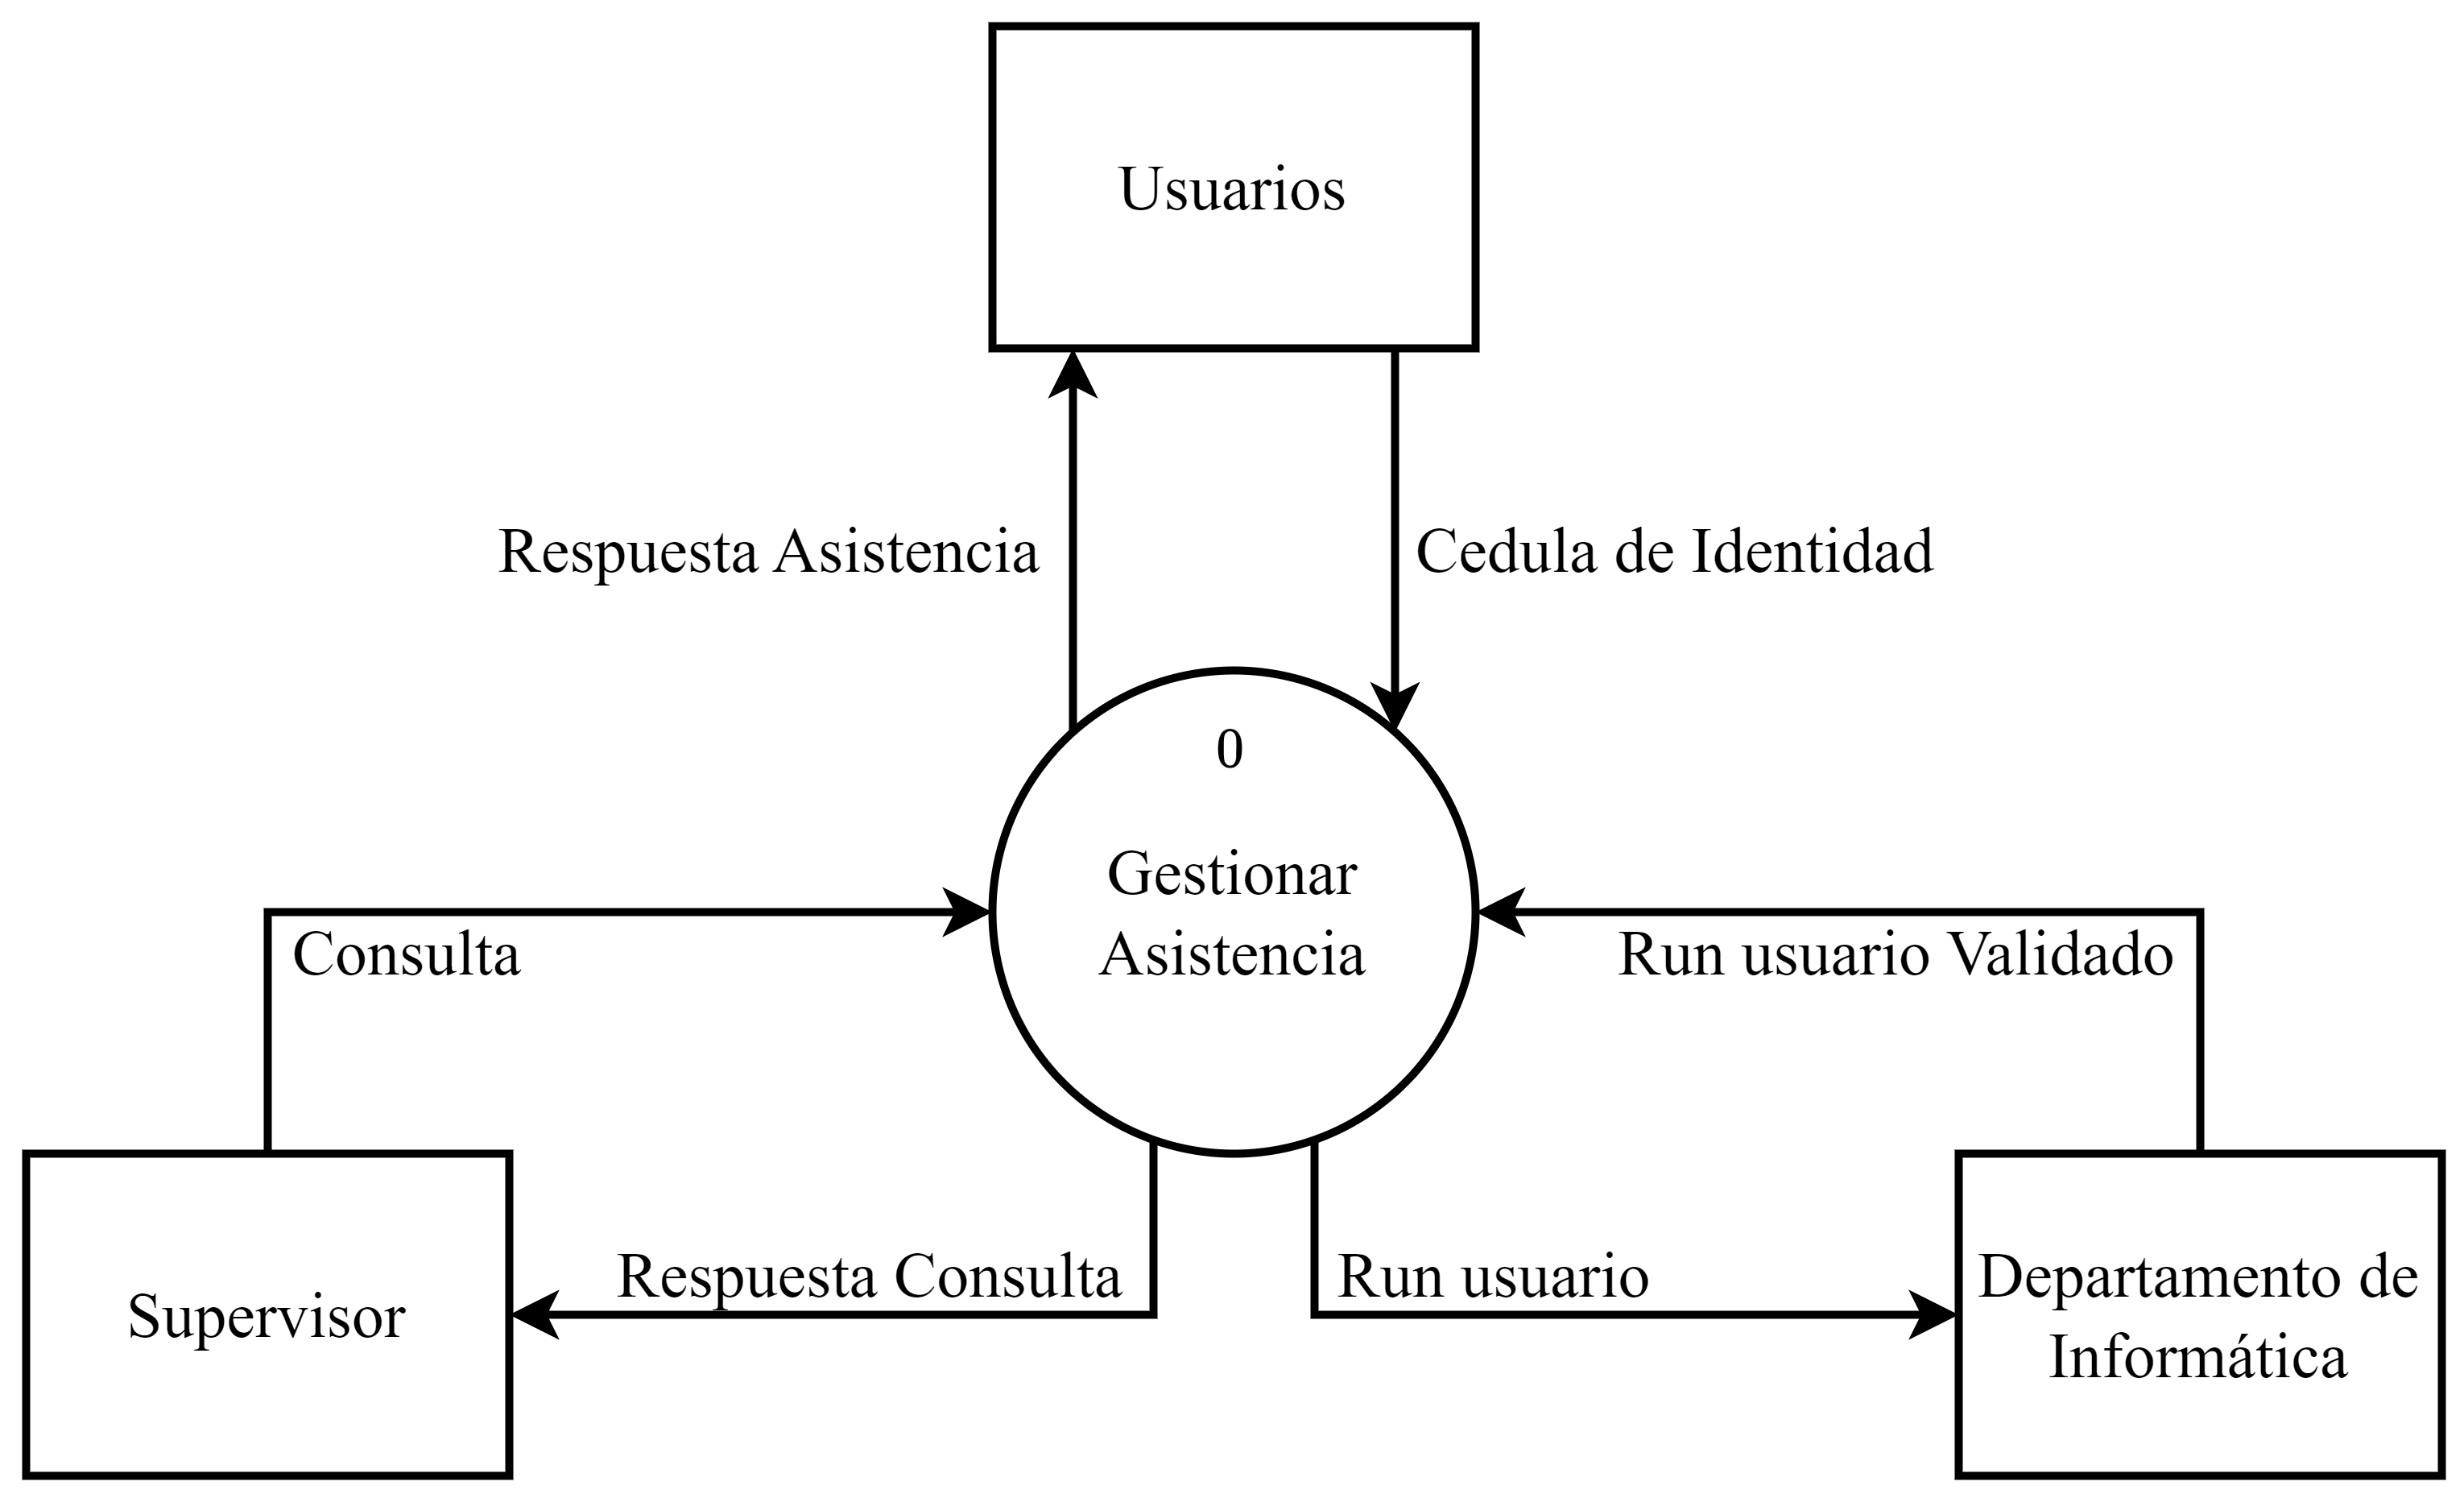
\includegraphics[scale=0.1]{img/TS-SI-Contexto.drawio.png}
    \caption{Diagrama de contexto}
    \label{fig:diagramaContexto}
\end{figure}
\subsection{Diagrama de nivel superior}
\begin{figure}[H]
    \centering
    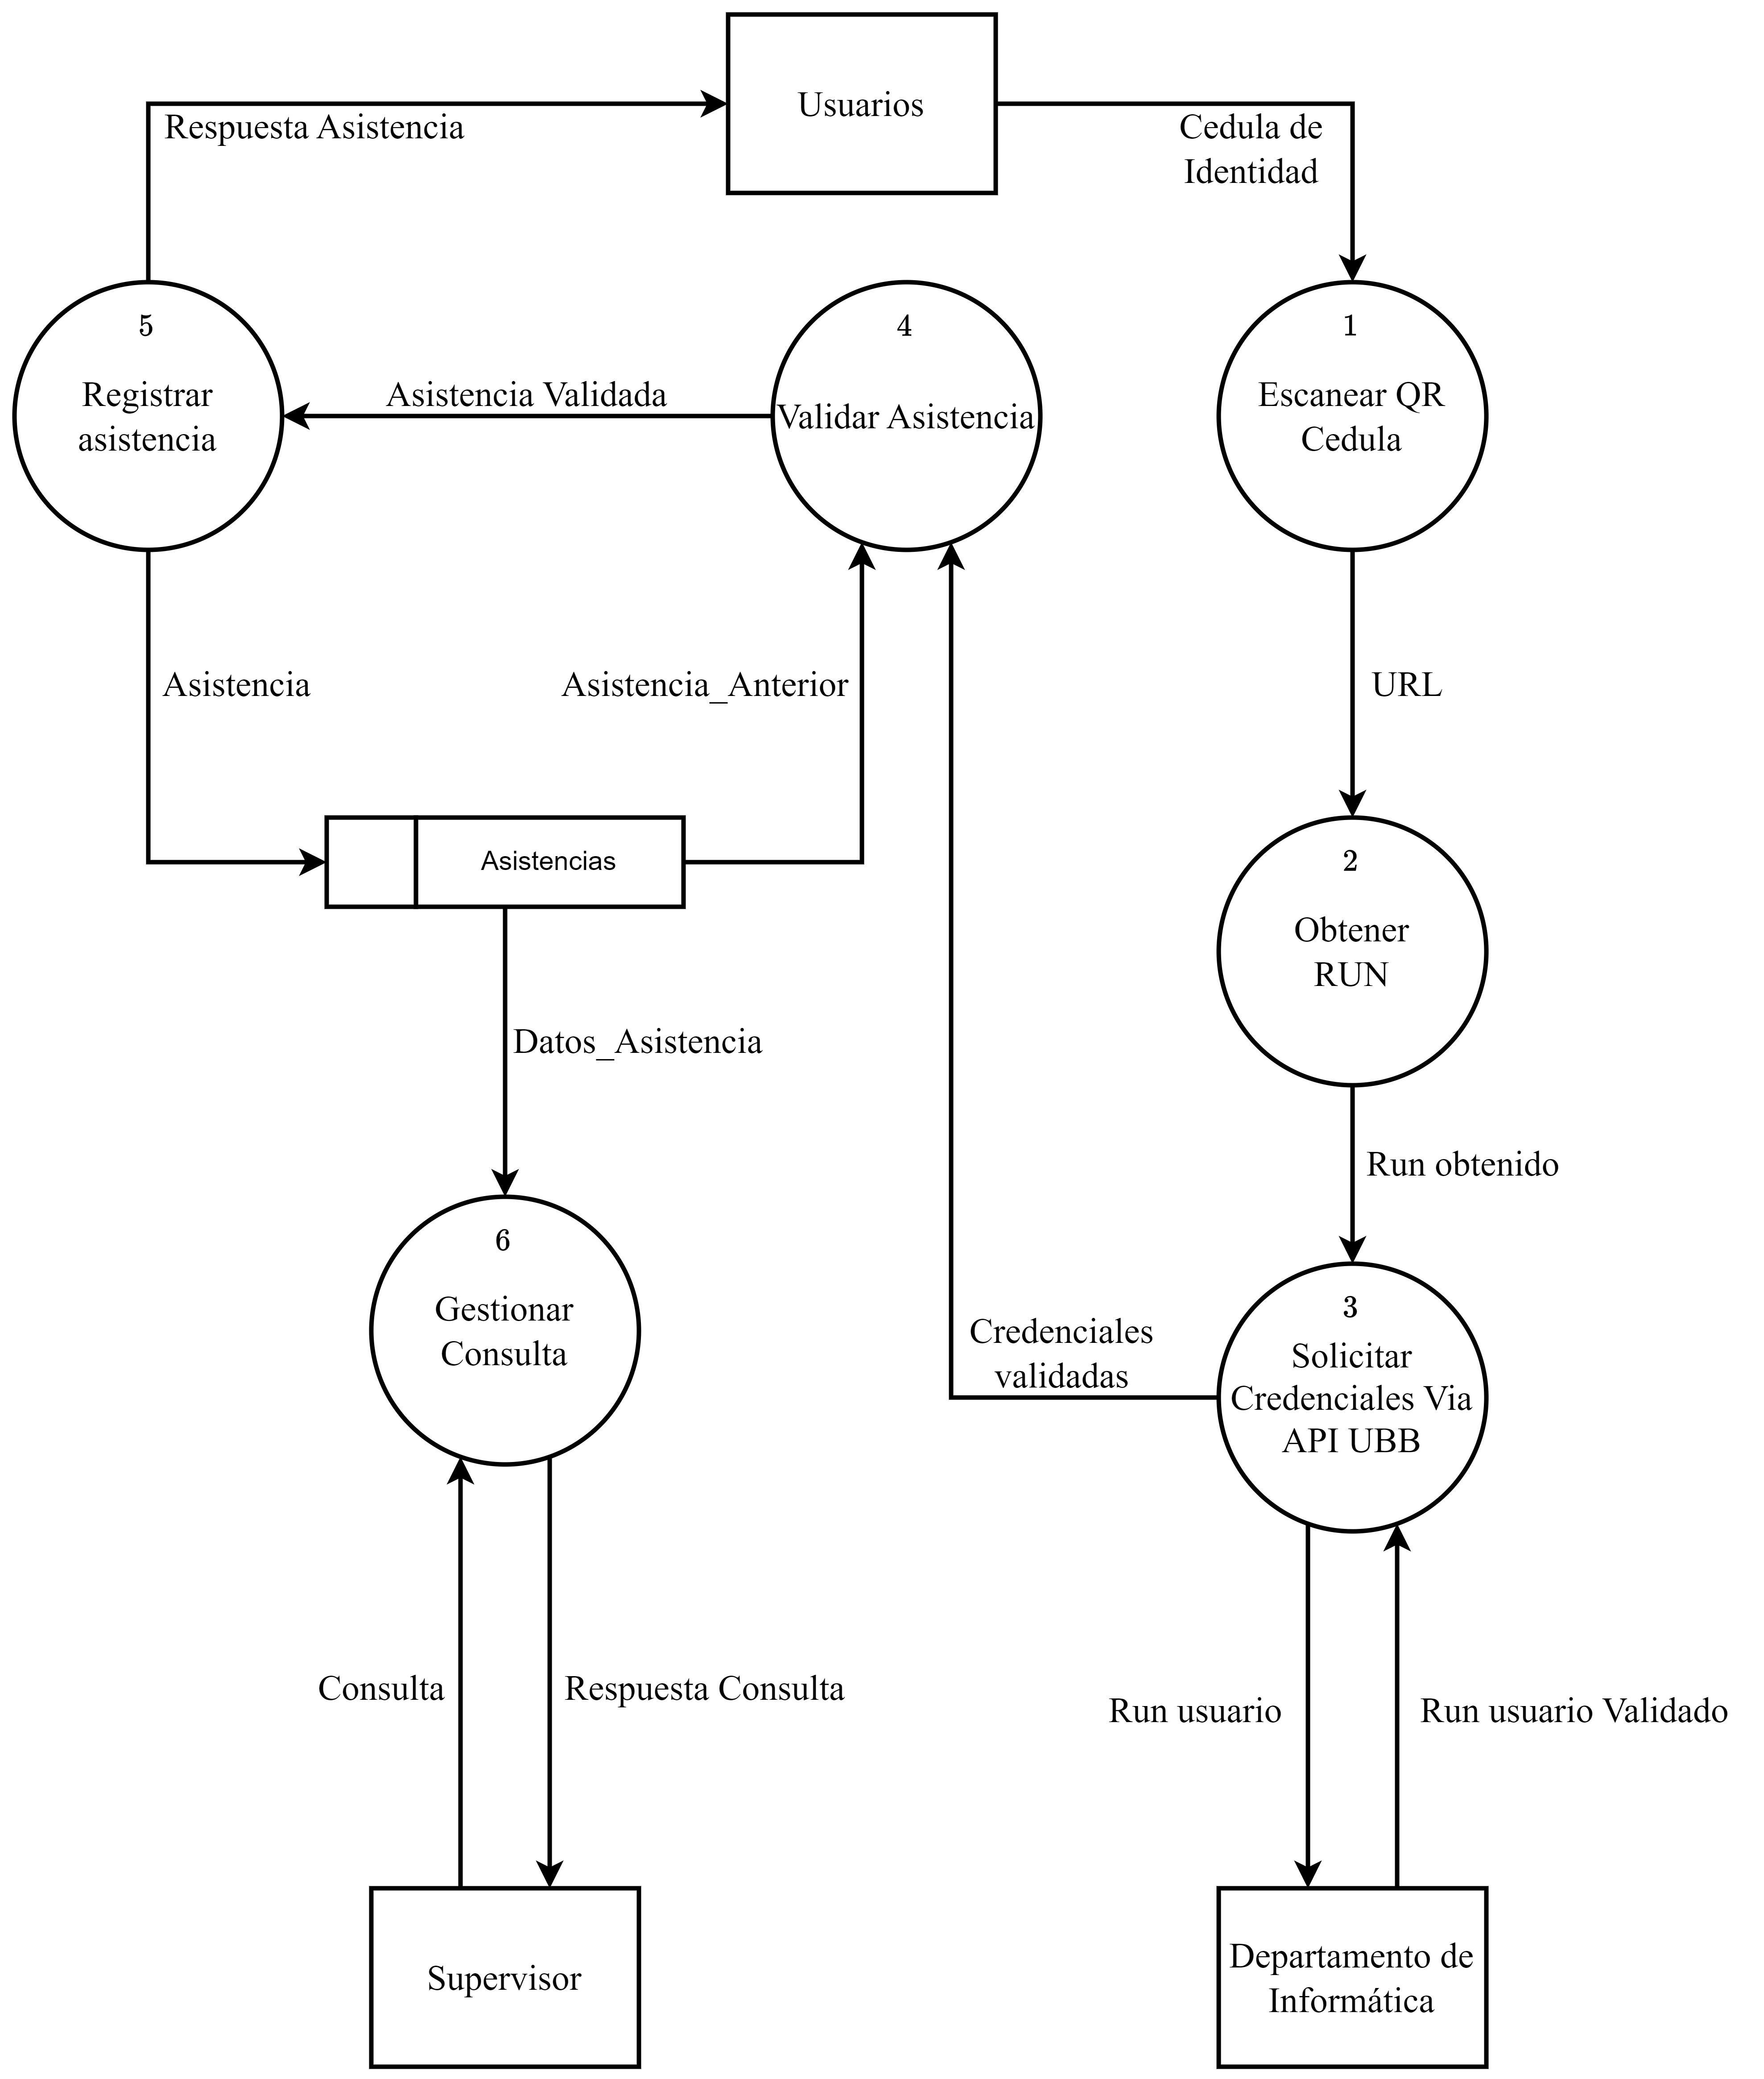
\includegraphics[scale=0.1]{img/TS-SI-Nivel Superior.drawio.png}
    \caption{Diagrama de nivel superior}
    \label{fig:diagramaNivelSuperior}
\end{figure}

\subsection{Procedimientos administrativos}
\begin{figure}[H]
    \centering
    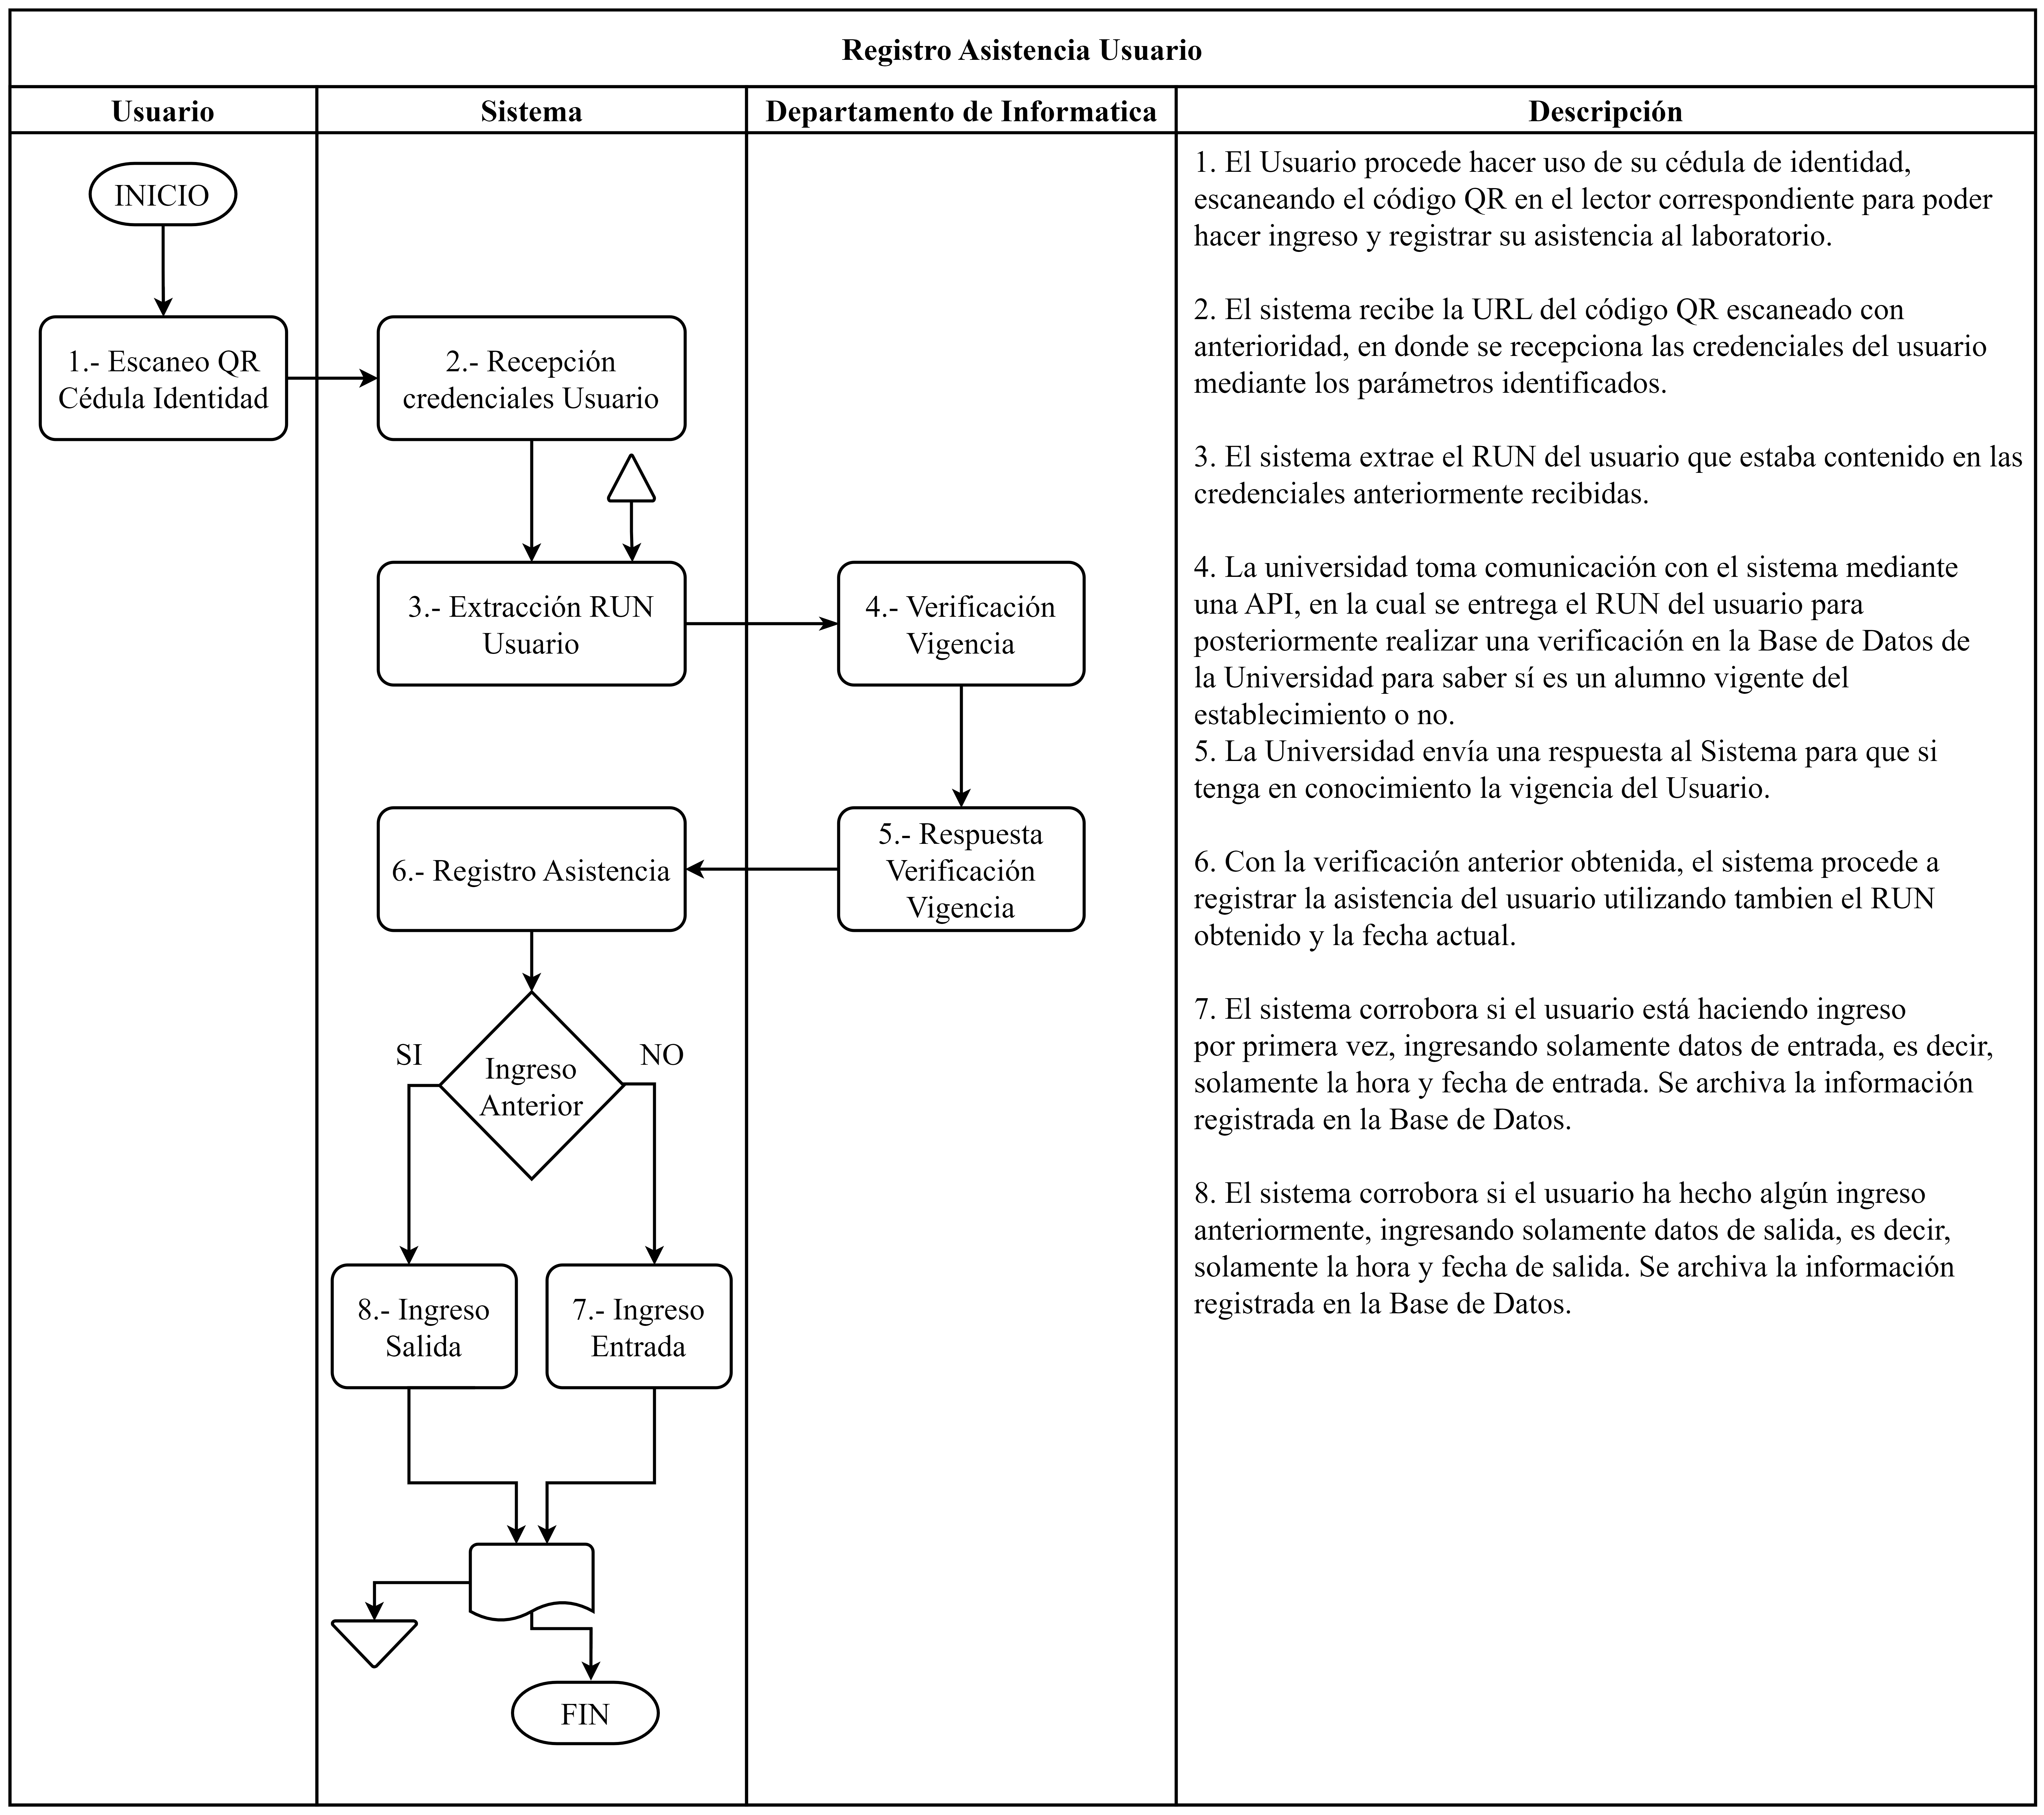
\includegraphics[scale=0.06]{img/TS-SI-Procedo Administrativo.drawio.png}
    \caption{Procedimientos administrativos}
    \label{fig:procedimientosAdministrativos}
\end{figure}

\newpage
\section{Etapa 1}
En esta etapa se desarrolló el sistema, registrando la fecha y hora del dispositivo en el que se ejecuta el programa, run del usuario. Se utilizó una base de datos local para almacenar los datos registrados.
\newpage
\begin{thebibliography}{99}
    \bibitem{ubb} Universidad del Bío-Bío \url{https://www.ubiobio.cl/w/}
\end{thebibliography}
\end{document}